


%_______________
\newpage\subsection*{Exercises} % Types of outliers in linear regression

% 1

\eoce{\qt{Outliers, Part I\label{outliers_1}} Identify the outliers in the 
scatterplots shown below, and determine what type of outliers they are. 
Explain your reasoning.
\begin{center}
\includegraphics[width=0.32\textwidth]{ch_regr_simple_linear/figures/eoce/outliers_1/outliers_1_influential.pdf}
\includegraphics[width=0.32\textwidth]{ch_regr_simple_linear/figures/eoce/outliers_1/outliers_2_leverage.pdf}
\includegraphics[width=0.32\textwidth]{ch_regr_simple_linear/figures/eoce/outliers_1/outliers_3_outlier.pdf}
\end{center}
}{}

% 2

\eoce{\qt{Outliers, Part II\label{outliers_2}} Identify the outliers in the scatterplots 
shown below and determine what type of outliers they are. Explain 
your reasoning.
\begin{center}
\includegraphics[width=0.32\textwidth]{ch_regr_simple_linear/figures/eoce/outliers_2/outliers_1_influential.pdf}
\includegraphics[width=0.32\textwidth]{ch_regr_simple_linear/figures/eoce/outliers_2/outliers_2_influential.pdf}
\includegraphics[width=0.32\textwidth]{ch_regr_simple_linear/figures/eoce/outliers_2/outliers_3_outlier.pdf}
\end{center}
}{}

% 3

\eoce{\qt{Urban homeowners, Part I\label{urban_homeowners_outlier}} The 
scatterplot below shows the percent of families who own their 
home vs. the percent of the population living in urban areas.
\footfullcite{data:urbanOwner} There are 52 observations, each 
corresponding to a state in the US. Puerto Rico and District of 
Columbia are also included.

\noindent\begin{minipage}[c]{0.5\textwidth}
\begin{parts}
\item Describe the relationship between the percent of families who 
own their home and the percent of the population living in urban areas.
\item The outlier at the bottom right corner is District of Columbia, 
where 100\% of the population is considered urban. What type of an outlier 
is this observation?
\end{parts}
\end{minipage}
\begin{minipage}[c]{0.05\textwidth}
$\:$\\
\end{minipage}
\begin{minipage}[c]{0.4\textwidth}
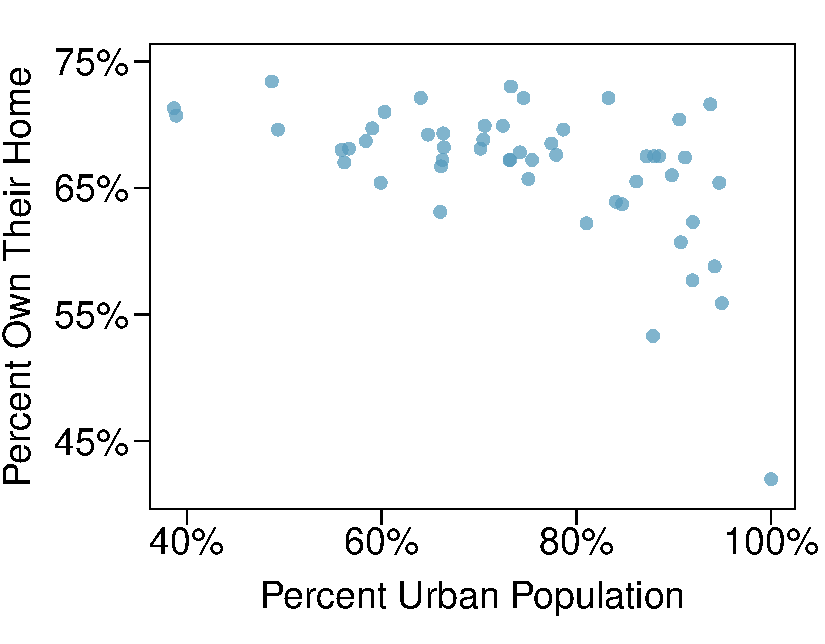
\includegraphics[width=0.95\textwidth]{ch_regr_simple_linear/figures/eoce/urban_homeowners_outlier/urban_homeowners_outlier.pdf} \vspace{-3mm}
\end{minipage}
}{}

% 4

\eoce{\qt{Crawling babies, Part II\label{crawling_babies_outlier}} 
Exercise~\ref{crawling_babies_corr_units} introduces 
data on the average monthly temperature during the month babies first 
try to crawl (about 6 months after birth) and the average first 
crawling age for babies born in a given month. A scatterplot of these 
two variables reveals a potential outlying month when the average 
temperature is about 53\degree F and average crawling age is about 
28.5 weeks. Does this point have high leverage? Is it an influential 
point?
}{}
